%\documentclass[wrr]{agutex}
\documentclass[wrr, draft]{agutex}
% Author names in capital letters:
\authorrunninghead{THORARINSDOTTIR ET AL.}

% Shorter version of title entered in capital letters:
\titlerunninghead{ADAPTING TO UNCERTAIN SEA LEVEL RISE}

%Corresponding author mailing address and e-mail address:
\authoraddr{Corresponding author: Name, Address. (email)}

\usepackage{bbm, amsmath}
%\usepackage[dvips]{graphicx}
\usepackage{graphicx}
\setkeys{Gin}{draft=false}
\usepackage{paralist, booktabs}
\usepackage{url}
\usepackage{color}


\usepackage{lineno}
 \linenumbers*[1]
%  To add line numbers to lines with equations:

\begin{document}

%% ------------------------------------------------------------------------ %%
%  TITLE
%% ------------------------------------------------------------------------ %%

\title{I don't know, are you sure we want to do this?\
Sea level adaptation decisions under uncertainty}

%% ------------------------------------------------------------------------ %%
%  AUTHORS AND AFFILIATIONS
%% ------------------------------------------------------------------------ %%

% \altaffilmark will produce footnote;
% matching \altaffiltext will appear at bottom of page.

\authors{T. Thorarinsdottir\altaffilmark{1}, P. Guttorp\altaffilmark{1}, M. Drews\altaffilmark{2}}

\altaffiltext{1}{Norwegian Computing Centere}

\altaffiltext{2}{Technical University of Denmark}

\altaffiltext{3}{Affiliation three}

%% ------------------------------------------------------------------------ %%
%  ABSTRACT
%% ------------------------------------------------------------------------ %%

\begin{abstract}
...
\end{abstract}


%% ------------------------------------------------------------------------ %%
%  BEGIN ARTICLE
%% ------------------------------------------------------------------------ %%

\begin{article}



\section{Introduction}\label{sec:intro}

\section{Sea level projections {\color{blue} (PG)}}



\subsection{Global sea level}
Most climate models do not explicitly provide sea level as an output of the calculations. Rather, the IPCC AR5 report \citep[ch.~13]{ipcc} combines the heat expansion of the ocean with temperature forced models for glacial melt, Greenland ice melt, and Antarctic ice melt and with land rise due to rebound from the last ice age. Judging from the supplementary material to \citet[ch.~13]{ipcc}, the uncertainty assessment is only based on the spread of the ensemble of temperature projections, not on the additional uncertainty in the ice models used.

We will instead use the empirical approach of Rahmstorf and collaborators \citep{Rahmstorf07,Rahmstorf11}, employing the statistical modeling of \citet{Bolin2014a} to relate global annual mean temperature anomalies \citep{giss} to global mean sea level anomalies \citep{csiro}. 
%Figure showing historical relationship?

We then apply the estimated historical relationship to projected temperatures from the CMIP5 experiment \citep{cmip5} to obtain projected global annual mean sea level, taking into account the uncertainty in the statistical model as well as the spread of the temperature projection ensemble (see subsection \ref{unc_ass}). 
For the i'th temperature projection $T_t^i$ we estimate the corresponding global mean sea level as

\[H_t^{gl,i} = \int\limits_{{t_0}}^t {{\hat a} (T_u^i - {{\hat T}_0}} )du + {\varsigma _t}\]
where ${\hat a}$ and ${\hat T}_0$ are regression parameters of observed global sea level on observed global temperature and $\varsigma_t$ the integrated time series regression error.

%Figure with sea level projections & IPCC projections?


\subsection{Local sea level}
In order to get from global sea level projections to local ones, it is important to note that sea level rise not is uniform over the globe. Glacial and land ice melting affect the local sea level differently depending on where the melted ice is located.
%Gravitaional effects
Another major effect in Fennoskandia is the land rise due to isostatic rebound from the glaciers of the last ice age. 
Again, we will use historical data to relate global sea level to isostatically corrected local sea level using a time series regression model. Figure \ref{fig:obs} shows uncorrected and corrected Bergen sea level data, and the relationship between the corrected Bergen data and the global sea level data. The time series regression uses an ARMA(1,1)-model \citep{boxjenkins}.
\begin{figure}
\begin{center}
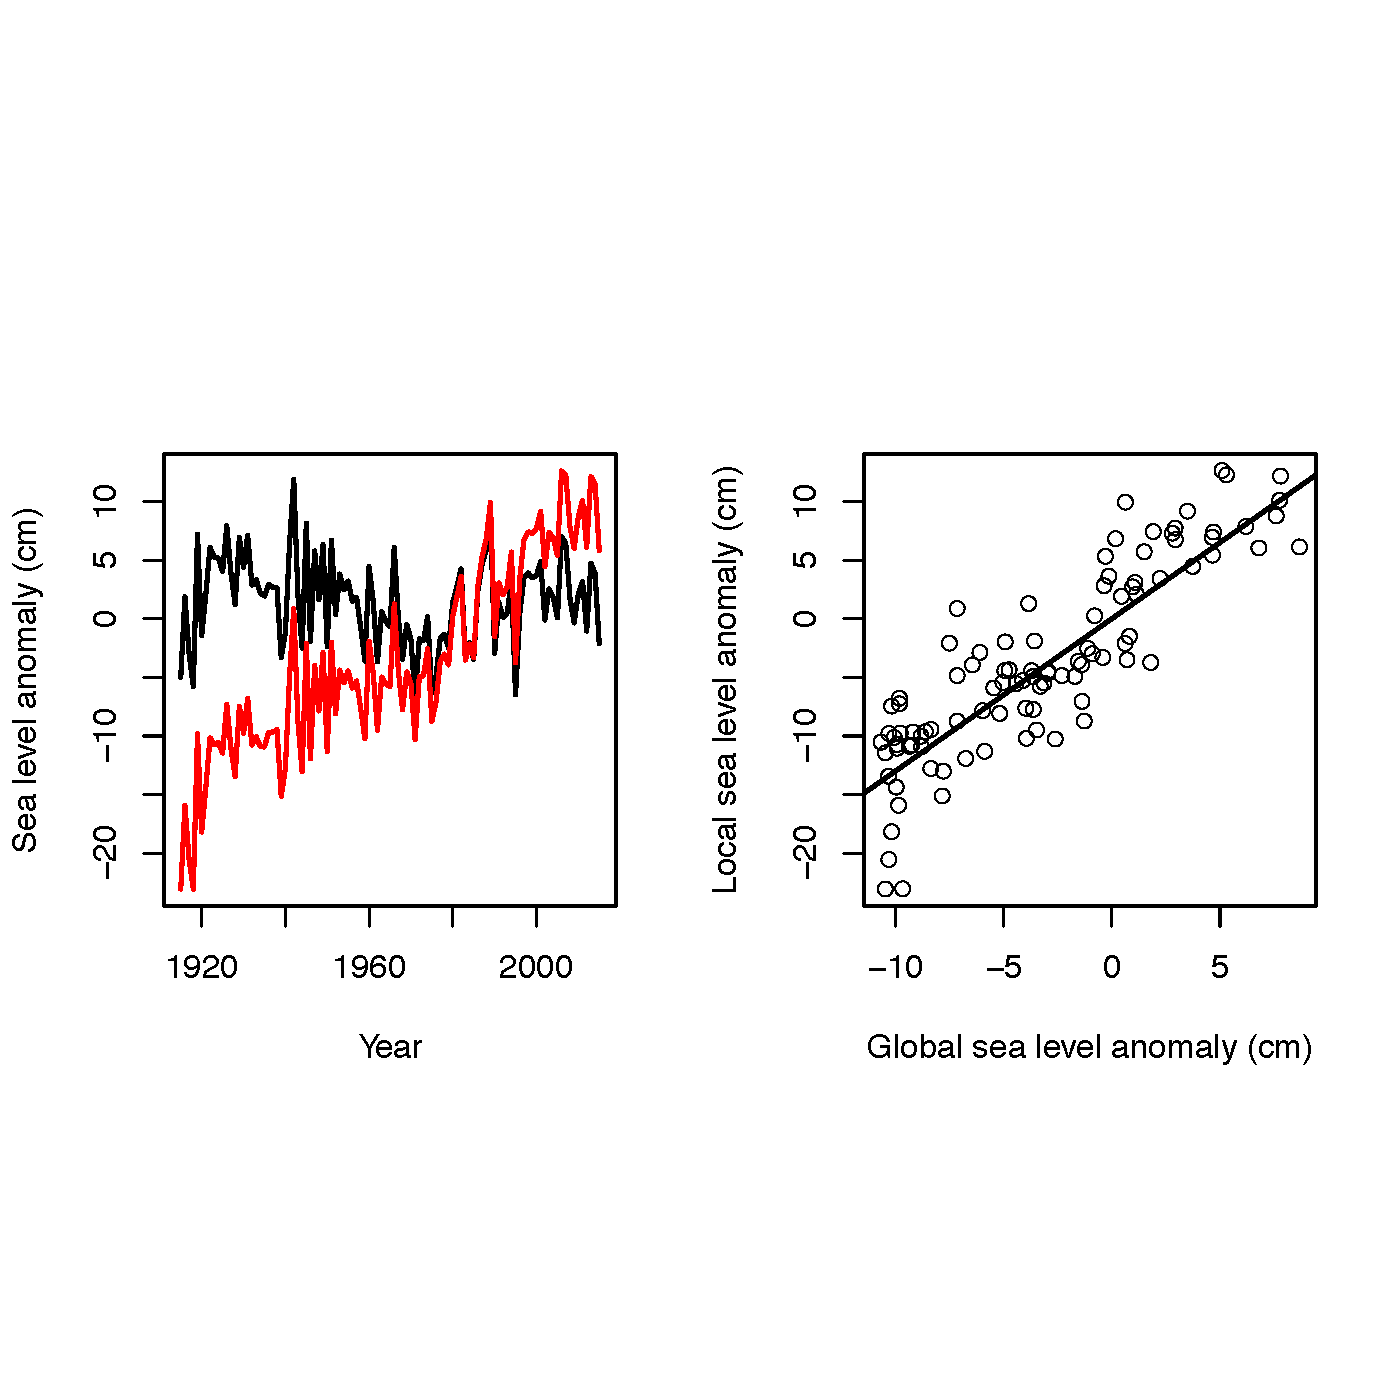
\includegraphics[width=39pc]{bergenfit.png}
\caption{ The left figure shows raw (black)and gia-corrected (red) sea level data from Bergen, The right figure relates the gia-corrected Bergen sea level to the global sea level series of \citet{csiro}. The straight line is the time series regression line.}
\label{fig:obs}
\end{center}
\end{figure}


The local sea level projections are then obtained by first relating projected temperature to global sea level, and then relating the global sea level to the local one. Each climate model temperature projection yields a different local sea level projection. The local sea level projection based on the i'th climate model for years beyond 2000 is estimated as

\[H_t^{loc,i} + \gamma (t -2000 ) = {\hat b} H_t^{gl,i}  + {\varepsilon _t}\]
where $\gamma$ ie the annual land rise rate, t and $ {\hat b} $ is the regression coefficient relating global to local sea level.



\subsection{Uncertainty assessment}
\label{unc_ass}
Following the approach of \citet{Guttorp2014} we assess the uncertainty in the local sea level projections taking into account the variability between the climate projections used, the uncertainties in the regressions of global mean temperature on global mean sea level and of global on local sea level. We express the sea level projection uncertainty in terms of a confidence band that is simultaneously of the intended  level  for all projection years. This allows us, for example, to get a confidence band for the years when a given sea level rise is obtained. 
\begin{figure}
\begin{center}
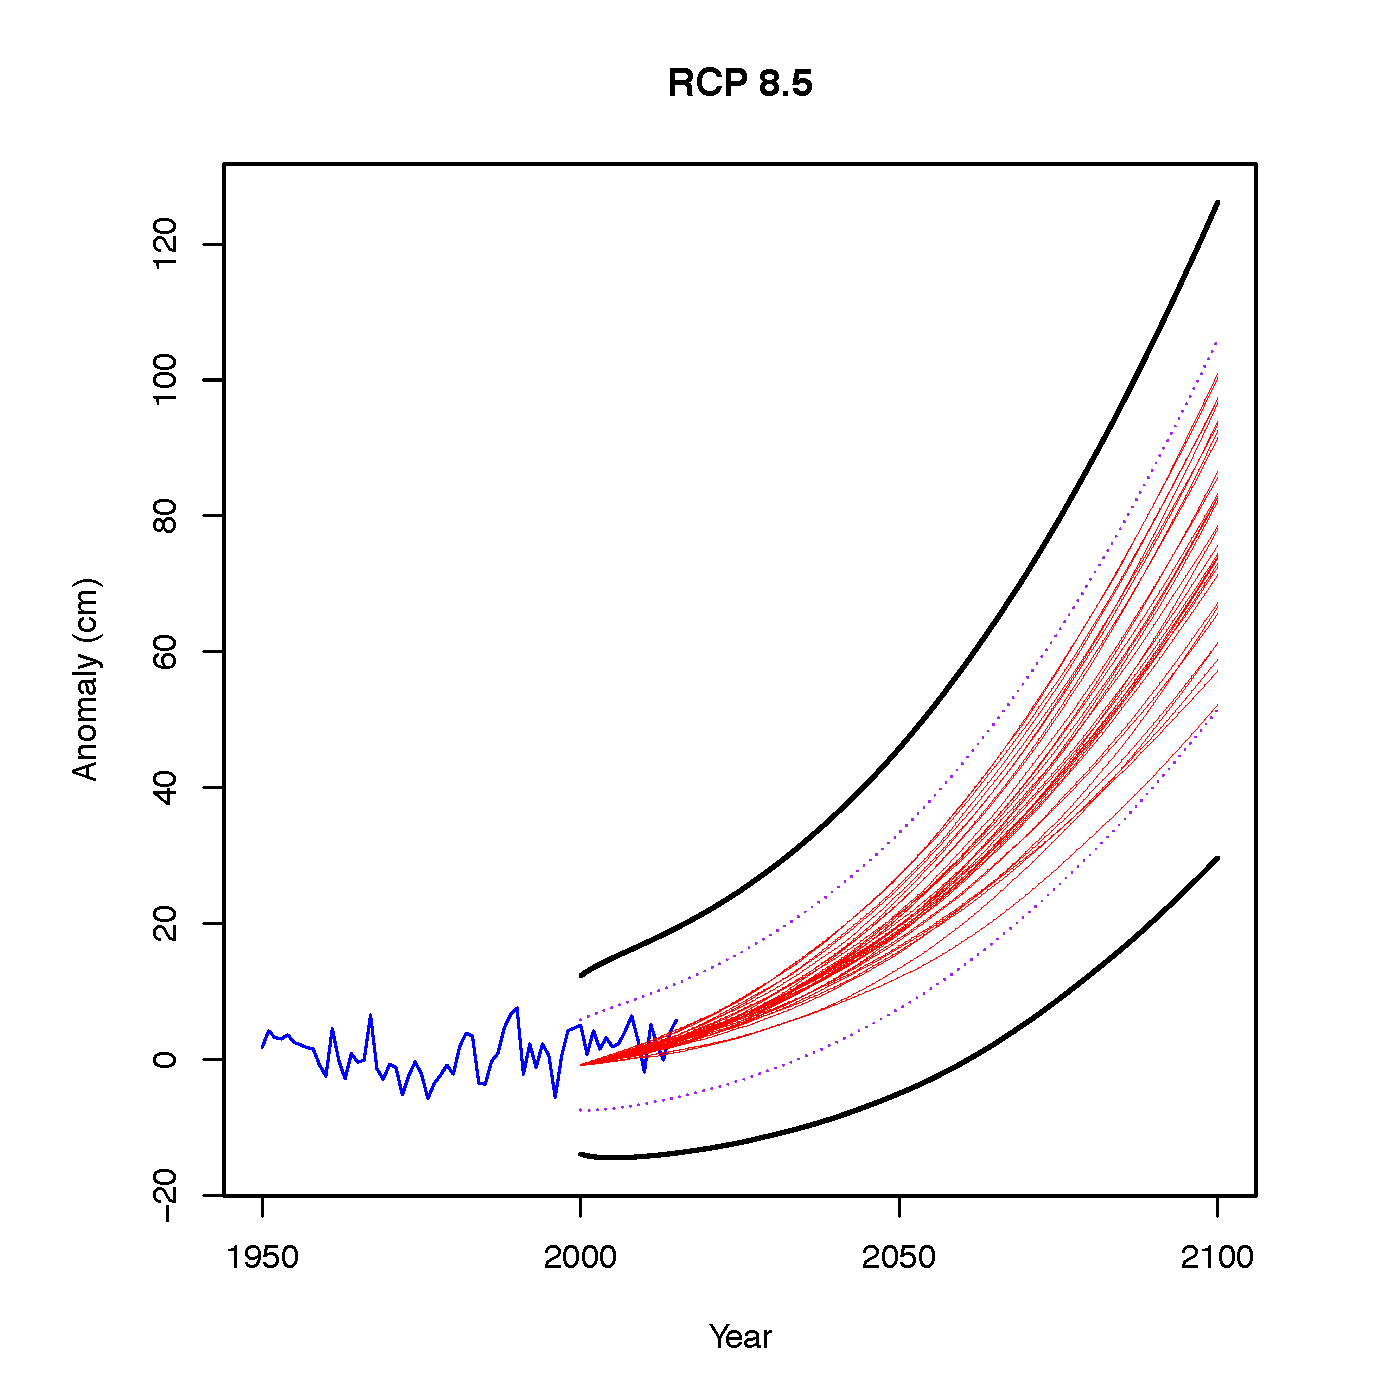
\includegraphics[width=39pc]{bergen_ci.png}
\caption{Simultaneous 90\% confidence set (thick black lines) for Bergen sea level projections for the years 2000-2100 using RCP8.5. The sea level data are shown in blue and end in 2015. The thin red lines are the projections without uncertainty based on each of the climate models. The dashed purple lines connect pointwise confidence intervals for each year. }
\label{fig:ci}
\end{center}
\end{figure}


\subsection{Limitations of the sea level projections}
The main assumption is using historical relationships in statistical projections of the type used in this paper is that there is no major change in how temperature relates to sea level, globally and locally. Among the factors that may invalidate this approach are changes in water storage on land (in essence removing water from the oceans), excessive siphoning of groundwater (resulting in land subsidence), changes in the rates of glacial and land ice melt, and changes in Earth's gravitational field due to transfer of mass from land ice to ocean water. For example, the rate of ice melt on Greenland may suddenly increase substantially due to intense warming of both air and sea water. Our current climate models are not able to resolve the ice processes sufficiently to include such so called tipping points into the projections. Also, the IPCC scenarios \citep{change} do not include changes in water usage.

\section{Decision tools {\color{blue} (KdB, MD, TT)}}

\subsection{Timing of adaptation measures}

We consider adaptation decision making related to the timing of proactive adaptation measures. That is, the goal is to adapt to sea level rise before major damages occur. In a cost-benefit framework, an investment should be delayed as long as the benefits of delay (avoided investment costs) are greater than the associated costs (higher climate change damages) \citep{Fankhauser&1999}.

\cite{Fankhauser&1999} describe a deterministic framework where an adaptation investment of $C^0$ now (at time $n=0$) leads to unmitigated damage of $d_0^0$ in period $0$, and a stream of partially mitigated damages $d_t^0$ in periods $t=1,2,\ldots$. If $r$ is the discount rate, the net present value damage, $D^0$, associated with this investment is
\begin{linenomath*}
\begin{equation}\label{eq:deterministic damage}
D^0 = C^0 + d_0^0 + \frac{d_1^0}{1+r} + \frac{d_2^0}{(1+r)^2} + \cdots  
\end{equation}
\end{linenomath*}
In comparison, postponing the adaptation investment to time period $n=1$ would lead to unmitigated damages in periods $0$ and $1$, and partially mitigated damages, $d_t^1$, thereafter. The delay would be preferable if
\begin{linenomath*}
\[
C^0 - \frac{C^1}{(1+r)} > (d_0^1 - d_0^0) + \frac{d_1^1 - d_1^0}{1+r} + \frac{d_2^1 - d_2^0}{(1+r)^2} + \cdots
\]
\end{linenomath*}
Here, the expression on the left describes the benefits of the delay while the expression on the right describes the cost of the delay. In the simplest case, there is no change in investment costs ($C^0 = C^1 = C$) and the delay has no lasting effects beyond period 1 ($d_t^1 = d_t^0$ for $t > 1$). In this case, the comparison is between the expected return $r$ earned on the captial while implementation is delayed and one addtional time period of unmitigated damage,
\begin{linenomath*}
  \[
  r C > d_1^1 - d_1^0.
  \]
  \end{linenomath*}

\subsection{Limitations of the decision framework}

\section{Case studies}

\subsection{Data {\color{blue} (PG)}}
We use local tide gauge data from the Permanent Service for Mean Sea Level, UK, which is the worldwide repository for national sea level data. Climate projections are from the fifth climate model intercomparison project, CMIP5. 

\subsection{Timing of adaptation measures {\color{blue} (KdB, TT)}}

A case study focusing on and comparing different cities in Norway.

\subsection{Selection of adaptation measures(?) {\color{blue} (MD)}}

A case study focusing on Denmark. 

\section{Conclusions}

%  ACKNOWLEDGMENTS
\begin{acknowledgments}
This work was funded by NordForsk through project number 74456 ``Statistical Analysis of Climate Projections'' (eSACP) and The Research Council of Norway through project number 243953 ``Physical and Statistical Analysis of Climate Extremes in Large Datasets'' (ClimateXL). The source code for the analysis is implemented in the statistical programming language {\tt R} (\url{http://www.R-project.org}) and is available on GitHub at \url{http://github.com/eSACP/...}.
\end{acknowledgments}

%%  REFERENCE LIST AND TEXT CITATIONS
% 5\bibliographystyle{../BibTeX/agufull08}
\bibliographystyle{agufull08}
\bibliography{ref.bib}
% Please use ONLY \citet and \citep for reference citations.

%\begin{thebibliography}{37}
%%   Before submitting: copy all the contents into the .bbl LaTeX file here
%%   and run latex again
%\providecommand{\natexlab}[1]{#1}
%\expandafter\ifx\csname urlstyle\endcsname\relax
%  \providecommand{\doi}[1]{doi:\discretionary{}{}{}#1}\else
%  \providecommand{\doi}{doi:\discretionary{}{}{}\begingroup
%  \urlstyle{rm}\Url}\fi


%\end{thebibliography}

%% ------------------------------------------------------------------------ %%
%  END ARTICLE
%% ------------------------------------------------------------------------ %%
\end{article}

%% Enter Figures and Tables here:

\end{document}
